\documentclass[12pt]{article}
\raggedbottom

\usepackage[utf8]{inputenc}
\usepackage{graphicx}
\usepackage[italian]{babel}
\usepackage{csquotes}
\usepackage{lipsum}
\usepackage{fancyhdr}
\usepackage{pdfpages}
\usepackage{wrapfig}
\usepackage{float}
\usepackage{enumitem}
\usepackage{subcaption}
\usepackage{framed}
\usepackage{listings,xcolor}
\usepackage{inconsolata}
\usepackage{setspace}
\usepackage{amsmath}
\usepackage[T1]{fontenc}
\usepackage[hidelinks]{hyperref}
\usepackage{booktabs}
\usepackage[a4paper,width=160mm,top=25mm,bottom=25mm]{geometry}

\definecolor{shadecolor}{gray}{0.8}

\title{\textbf{\textsc{Progetto 2}}\\Metodi del Calcolo Scientifico}

\author{Elisa Pioldi\\
        Mat. 856591}
\date{Giugno 2023}

\begin{document}

\maketitle

\section{Introduzione}

Il progetto qui presentato si compone di due parti:
\begin{enumerate}
    \item Implementazione della propria DCT2 (My DCT)
    \item Realizzazione di un software per convertire le immagini in formato BMP ad un formato compresso simil-JPEG (BMP converter)
\end{enumerate}

Tutte le risorse e il codice sorgente sono open-source disponibili al repository
\href{https://github.com/epi-xel/dct-compression}{\textit{epi-xel/dct-compression}}
su GitHub.

\section{My DCT}

Per l'implementazione e l'analisi dei tempi della propria DCT2, si è usufruito degli strumenti messi a disposizione di Jupyter, scrivendo il codice in Python.

Si sono pertanto utilizzate le liberie \texttt{numpy} per l'implementazione propria della DCT e \texttt{scipy.fftpack} per l'utilizzo della DCT fast già implementata. La libreria in particolare forniva solo la DCT applicabile a vettori, si è quindi implementata la DCT2 in un metodo a parte. Per ottenere lo scaling opportuno, è stato necessario passare nel metodo il parametro \texttt{norm='ortho'}.

Relativamente ai grafici si è fatto uso delle librerie \texttt{matplotlib}, \texttt{pandas} e \texttt{seaborn}; infine dato che l'esecuzione degli algoritmi su matrici molto grosse era computazionalmente molto pesante, si sono utilizzate alcune librerie per implementare una parallelizzazione dell'esecuzione degli algoritmi sulle matrici di test.

Il notebook è strutturato in modo tale da mantenere le varie funzionalità divise tra loro, con alcuni metodi per la generazione di matrici.

Si è quindi scritto il codice per eseguire la propria DCT, applicando la formula della DCT di tipo II per ricavare i coefficienti della nuova base:

\[
    c_k = \alpha_{k}^{N} \sum\limits_{i=0}^{N-1} f_i \cos \biggl(\pi k \dfrac{2i+1}{2N} \biggl), \quad k = 0, ..., N-1
\]
dove $\alpha_{k}^{N} = \frac{1}{\Vert w_k \Vert}$ è il fattore di normalizzazione:

\[
\alpha_{k}^{N}=
\begin{cases}
\frac{1}{\sqrt{N}} & \text{se } k=0 \\
\sqrt{\frac{2}{N}} & \text{se } k\neq0
\end{cases}
\]

\begin{figure}[!ht]
    \begin{center}
    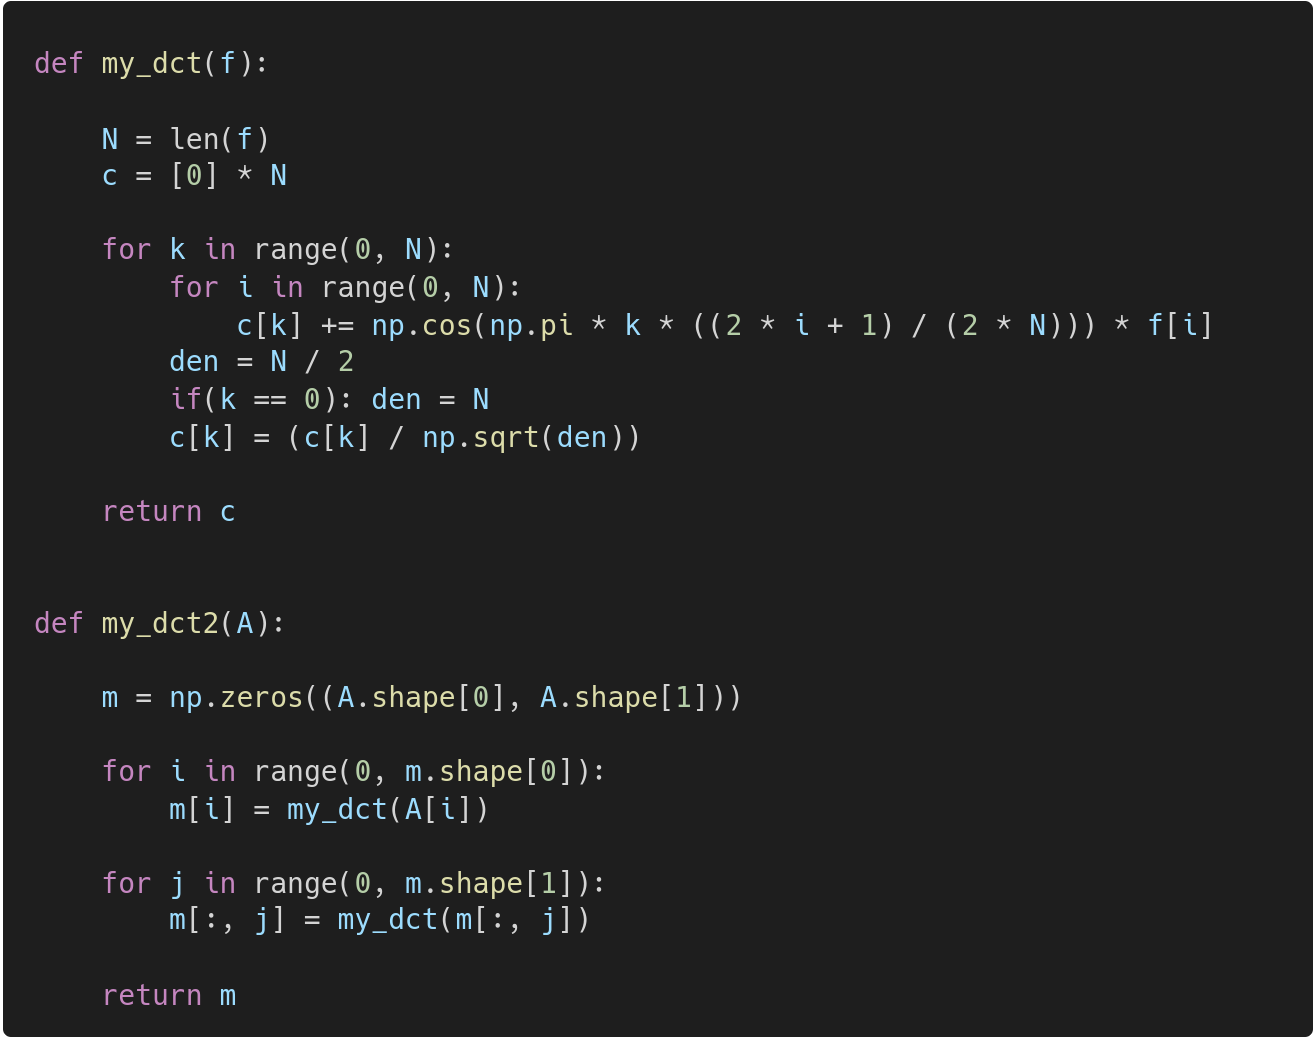
\includegraphics[scale=0.3]{images/code_mydct.png}
    \caption{Implementazione della My DCT2.}
    \end{center}
\end{figure}

Una volta implementati i metodi per il calcolo della DCT su matrici, si sono prodotte una serie di matrici di test, generate con numeri casuali da 0 a 255.

Si sono poi eseguiti entrambi gli algoritmi sulle matrici di test parallelizzandoli, e si sono infine prodotti i grafici relativi ai tempi.

\paragraph{Studio del limite superiore}
Come prima cosa si è voluto osservare la crescita del tempo computazionale. Banalmente nell'implementazione dell'algoritmo osserviamo nella DCT un doppio ciclo da 1 a N, che porta quindi a $O(n^2)$, tempo che con la DCT2 che viene applicata prima a righe poi a colonne si alza fino a $O(n^3)$.

Si sono quindi prodotte delle matrici dalla dimensione di $2 \times 2$ fino a $330 \times 330$, incrementando ogni volta la dimensione del lato di 2 unità (si noti che questi numeri sono stati scelti empiricamente osservando la capacità e i tempi computazionali della macchina su cui si stavano eseguendo gli algoritmi).

Possiamo osservare i risultati della computazione nella figura \ref{fig:2to330}, in scala semilogaritmica.

Analizzando i risultati \textit{My DCT} ha un andamento regolare di tipo polinomiale, come ci saremmo aspettati date le analisi preliminari.

La DCT fast presenta invece un profilo irregolare ma pur sempre polinomiale, anche se di ordine inferiore rispetto a \textit{My DCT}. Le diverse irregolarità sono dovute probabilmente alle ottimizzazioni implementate dalla libreria utilizzata.

\begin{figure}[!ht]
    \begin{center}
    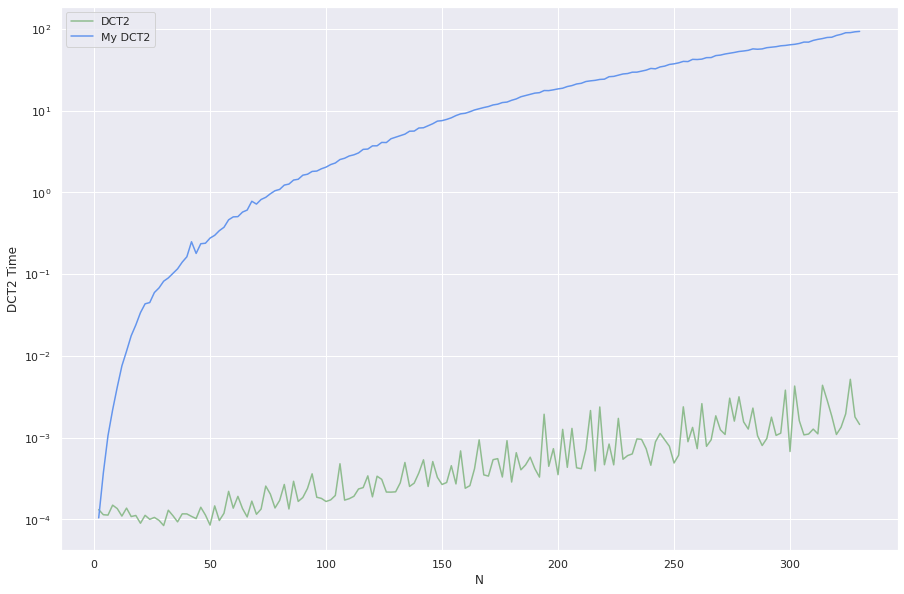
\includegraphics[scale=0.5]{images/2to330.png}
    \caption{Line-plot dei tempi calcolati in scala semilogaritmica.}
    \label{fig:2to330}
    \end{center}
\end{figure}

\paragraph{Studio del caso ottimizzato per la DCT fast}
Si rende necessario riportare alcune nozioni riguardanti l'algoritmo utilizzato per la DCT fast.
Quest'ultimo è infatti ottimizzato secondo un algoritmo divide-et-impera, ergo il caso in cui la grandezza del lato delle matrici è una potenza di 2 è il suo caso migliore. Le ottimizzazioni interne dovute a questo giustificano in parte l'andamento irregolare della curva, che vede una decrescita del tempo computazionale in corrispondenza delle dimensioni che rispondono bene alle divisioni per due.

\section{BMP converter}

La seconda parte del progetto vede l'implementazione di un'interfaccia grafica che, selezionata un'immagine BMP in toni di grigio, vi applica un algoritmo di compressione simil-jpeg ma senza utilizzare una matrice di quantizzazione.

\subsection{Librerie utilizzate}

Per l'implementazione del software per comprimere immagini BMP si è utilizzato sempre il linguaggio Python ma il codice è stato strutturato secondo un'architettura ben definita a moduli.

In particolar modo, l'interfaccia grafica si è ottenuta grazie a due librerie per GUI di Python: Tkinter e PyQt5. Per permettere a questi due librerie di lavorare insieme armoniosamento si sono utilizzate alcune librerie per la gestione di thread e processi. Relativamente al tema che è stato applicato all'interfaccia grafica di Tkinter, si è sfruttata una libreria open-source disponibile su GitHub al seguente repository: \href{https://github.com/rdbende/Sun-Valley-ttk-theme}{\textit{rdbende/Sun-Valley-ttk-theme}}. Inoltre l'applicazone è resa interamente responsive.

Il back-end è stato invece implementato con l'asilio delle librerie Numpy e FFTPACK di Scipy per l'elaborazione numerica e Pillow per la manipolazione di immagini.

\subsection{Back-end}

Lo sviluppo del modulo contenente le funzioni per la conversione dell'immagine è molto lineare.
Ci sono due metodi ausiliari che caricano dapprima l'immagine convertendola in una mappa di pixel e poi ancora in una matrice facilmente trattabile.

\begin{figure}[!ht]
    \begin{center}
    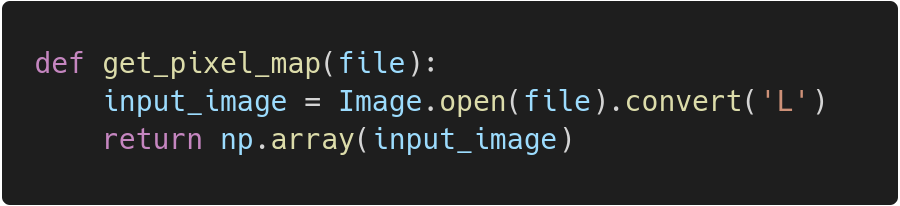
\includegraphics[scale=0.3]{images/code_get_pixel_map.png}
    \caption{Metodo per la conversione dell'immagine in una mappa di pixel.}
    \end{center}
\end{figure}

Il metodo principale prende in ingresso quindi la mappa di pixel e i parametri $F$ e $d$. 

\begin{figure}[!ht]
    \begin{center}
    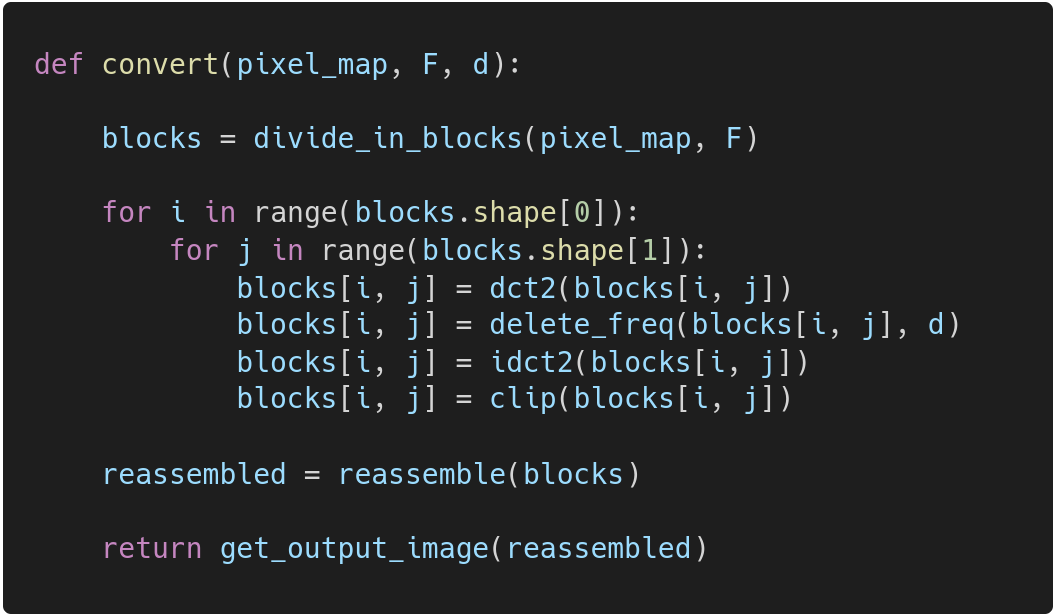
\includegraphics[scale=0.3]{images/code_convert.png}
    \caption{Metodo principale per la conversione.}
    \end{center}
\end{figure}

Al suo interno viene prima di tutto chiamato un metodo che divide l'immagine in blocchi, che consistono in piccole sottomatrici.

Per ogni blocco vengono poi applicate in sequenza DCT2, eliminazione delle frequenze, arrotondamento e normalizzazione dei valori e infine la DCT2 inversa (ciacuna di queste operazioni è definita in un metodo apposito).

\begin{figure}[!ht]
    \begin{center}
    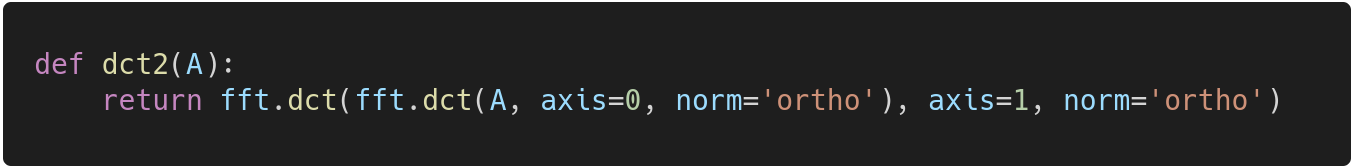
\includegraphics[scale=0.3]{images/code_dct2.png}
    \caption{Metodo per eseguire la DCT2.}
    \end{center}
\end{figure}

\begin{figure}[!ht]
    \begin{center}
    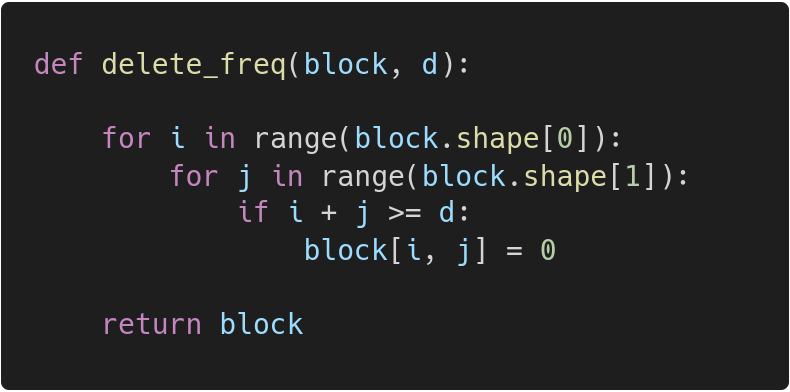
\includegraphics[scale=0.3]{images/code_delete_freq.png}
    \caption{Metodo per l'eliminazione delle frequenze.}
    \end{center}
\end{figure}

\begin{figure}[!ht]
    \begin{center}
    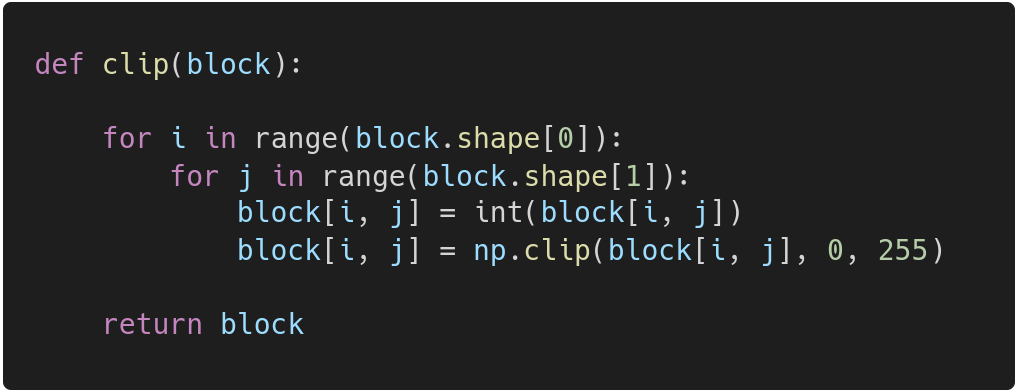
\includegraphics[scale=0.3]{images/code_clip.png}
    \caption{Metodo per l'arrotondamento e la normalizzazione.}
    \end{center}
\end{figure}

\begin{figure}[!ht]
    \begin{center}
    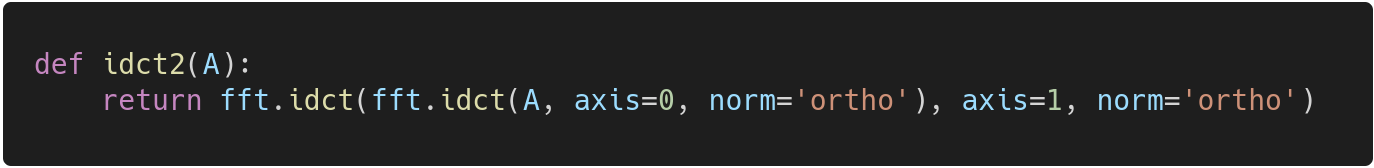
\includegraphics[scale=0.3]{images/code_idct2.png}
    \caption{Metodo per eseguire la DCT2 Inversa.}
    \end{center}
\end{figure}

Viene infine chiamato un metodo che assembla nuovamente i blocchi in ordine e riconverte la matrice in immagine.

\begin{figure}[!ht]
    \begin{center}
    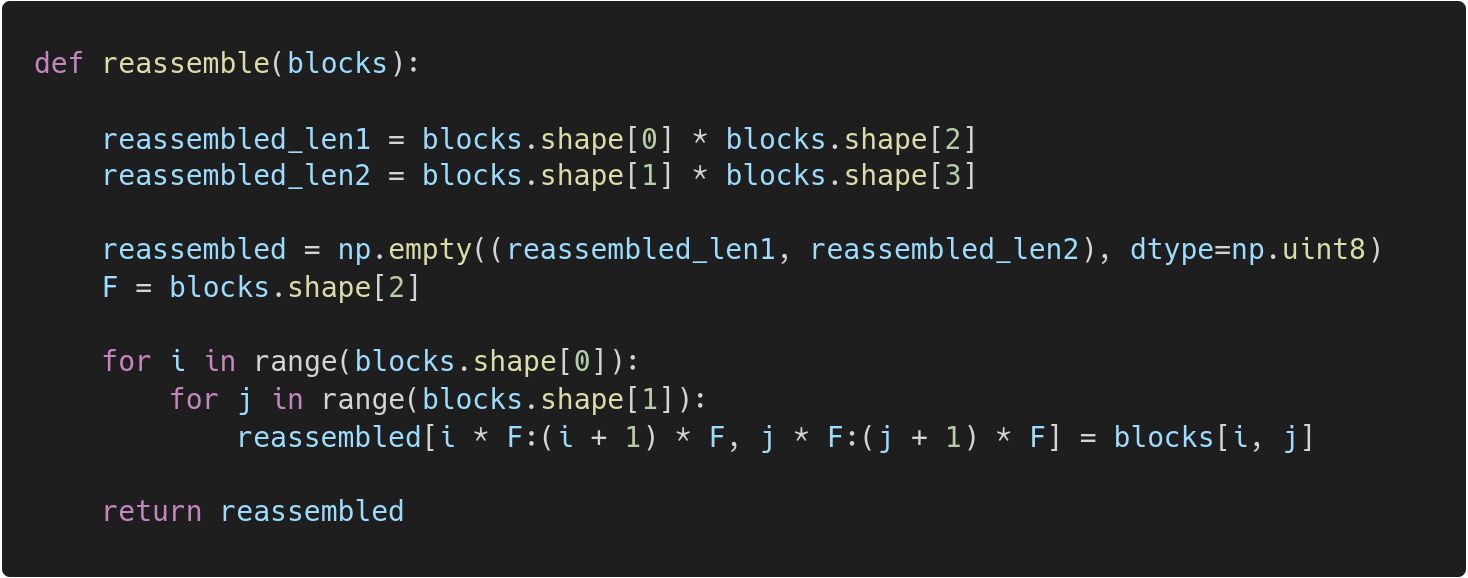
\includegraphics[scale=0.3]{images/code_reassemble.png}
    \caption{Metodo per assemblare i blocchi nella matrice originale.}
    \end{center}
\end{figure}

Si noti che si è deciso di scartare tutti i pixel sovrabbondanti nella divisione in blocchi.

\subsection{Front-end}

L'applicazione una volta eseguita presenta una prima finestra con alcune istruzioni sul funzionamento e un pulsante per scegliere il file, come si vede a figura \ref{fig:main}. 

\begin{figure}[!ht]
    \begin{center}
    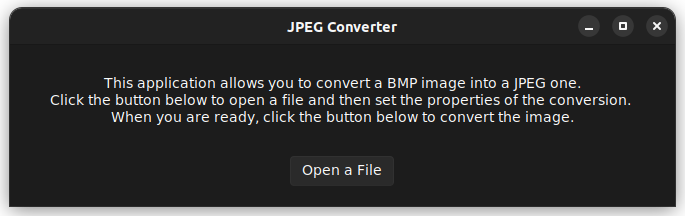
\includegraphics[scale=0.5]{images/main.png}
    \caption{Finestra principale dell'applicazione.}
    \label{fig:main}
    \end{center}
\end{figure}

Cliccando sul pulsante si apre una finestra con esplora risorse da cui si può selezionare il file BMP che si desidera convertire (figura \ref{fig:fc}). 

\begin{figure}[!ht]
    \begin{center}
    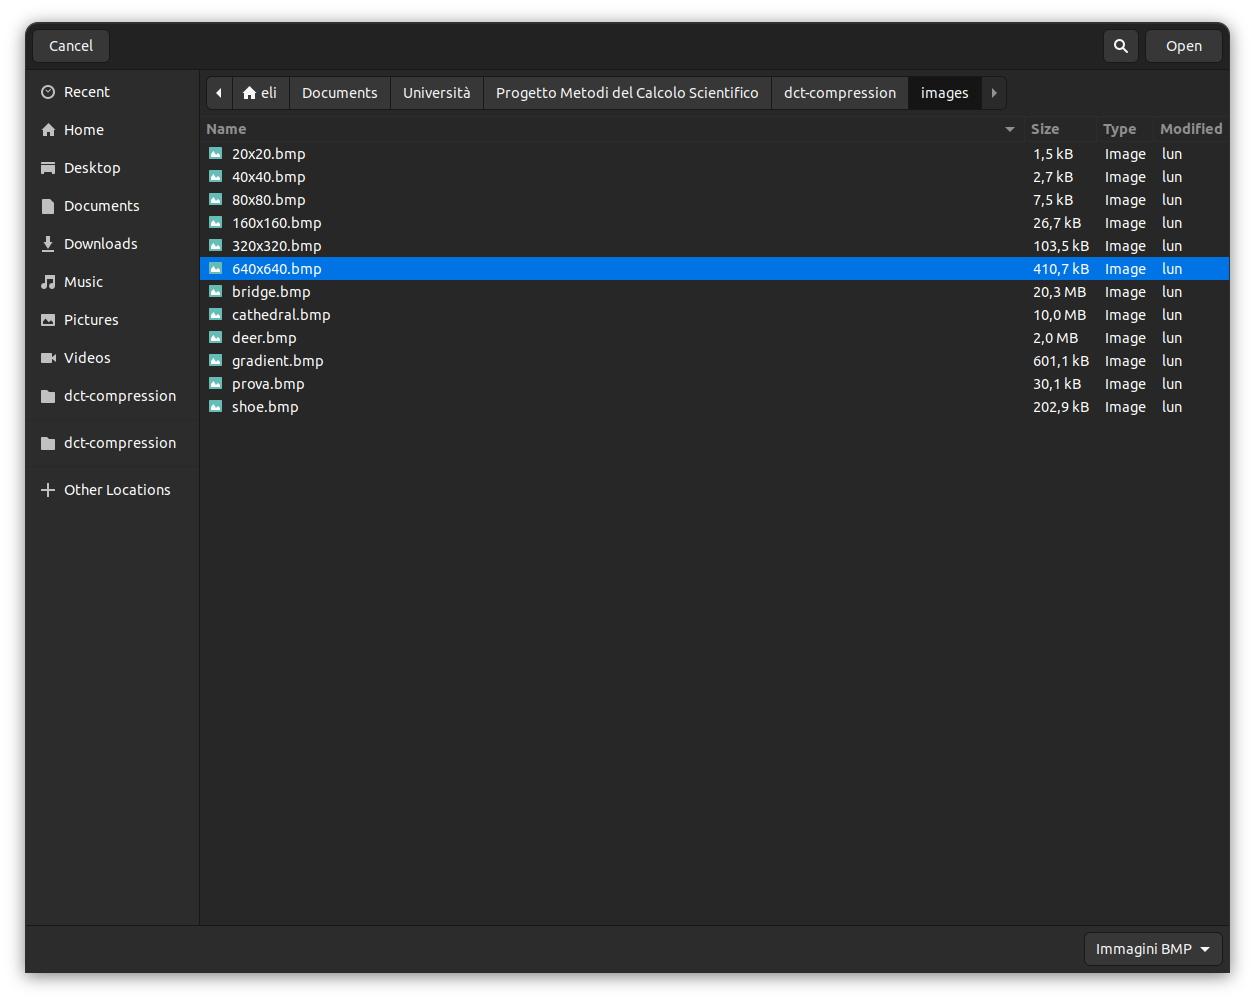
\includegraphics[width=\textwidth]{images/filechooser.png}
    \caption{Esplora risorse per selezionare il file.}
    \label{fig:fc}
    \end{center}
\end{figure}

Selezionando il file si ritorna alla finestra principale in cui è ora possibile visualizzare il file scelto (ed eventualmente fare zoom su di esso). Sotto l'immagine è quindi presente un panel con due \textit{scalebar} che permettono di impostare la dimensione dei macro-blocchi ($F$) e la soglia di taglio delle frequenze ($d$). Si è scelto si lasciare come valore massimo di F la lunghezza del lato più corto dell'immagine, mentre nell'interfaccia a seconda del valore F selezionato la \textit{scalebar} relativa a d si ridimensiona dinamicamente come valore massimo, settato a $2F-2$, come si può osservare nella figura \ref{fig:tune}.

\begin{figure}[!ht]
    \begin{center}
    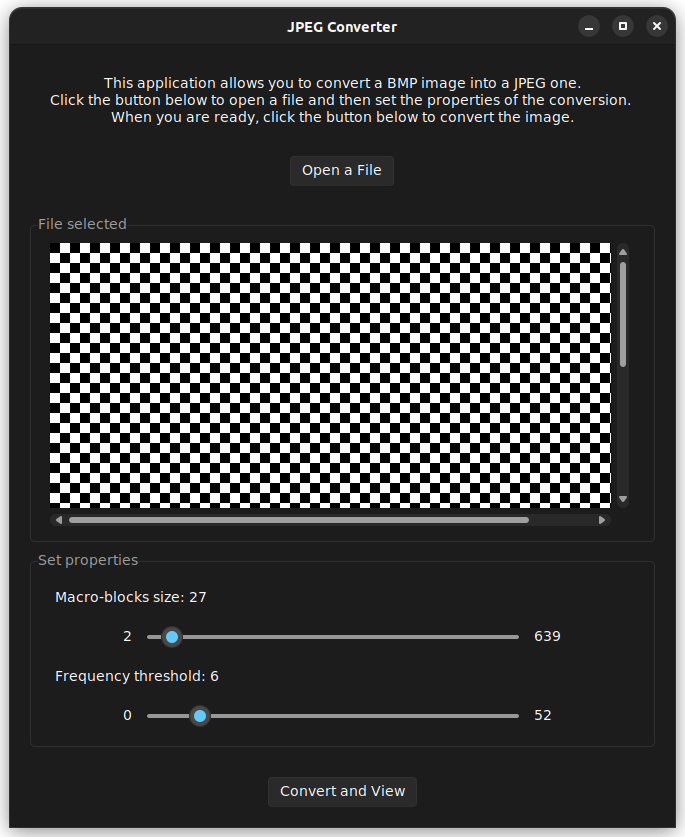
\includegraphics[scale=0.4]{images/tune.png}
    \caption{Visualizzazione della finestra dopo aver scelto il file e impostato i parametri.}
    \label{fig:tune}
    \end{center}
\end{figure}

Una volta settati i parametri desiderati cliccando sul pulsante in basso \textit{Convert} dopo qualche secondo si aprirà una finestra contenente le due immagini una vicino all'altra, su cui è possibile effettuare uno zoom e spostamento congiunto (si veda figura \ref{fig:comp}).

Se si vuole convertire un'altra immagine o convertire la stessa ad un'altra risoluzione, l'applicazione è strutturata in modo tale da poter lasciare aperta la finestra per il confronto.

\begin{figure}[!ht]
    \begin{center}
    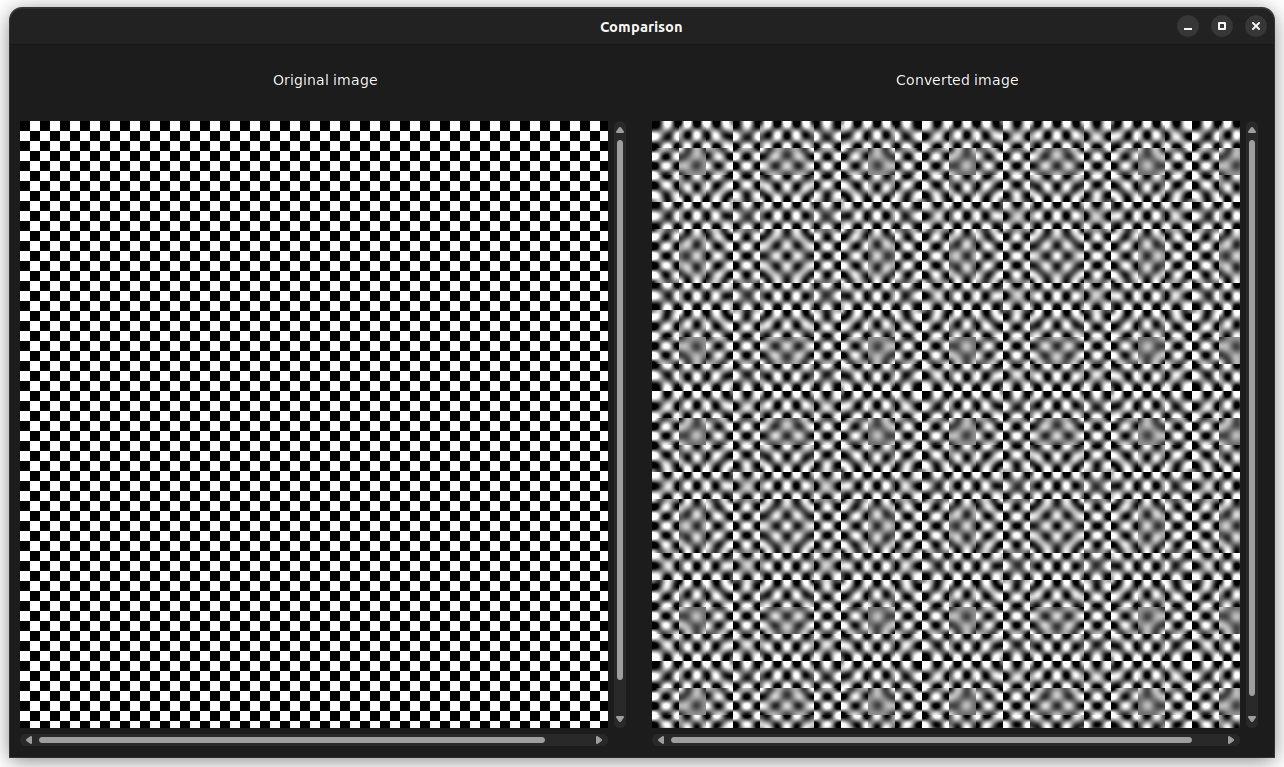
\includegraphics[width=\textwidth]{images/comparison.png}
    \caption{Confronto tra l'immagine originale e convertita.}
    \label{fig:comp}
    \end{center}
\end{figure}

\subsection{Considerazioni}

Osserviamo come cambia l'immagine compressa rispetto alla grandezza dei blocchi e della soglia di taglio delle frequenze.

Se si imposta come grandezza del blocco 8, come accade nella compressione JPEG standard, analizziamo come cambia incrementando man mano la soglia di taglio delle frequenze.

Impostando $d$ a 0, otteniamo un'immagine completamente nera, poiché non viene mantenuta nessuna informazione dell'immagine originale (cfr. figura \ref{fig:d80})

\begin{figure}[!ht]
    \begin{center}
    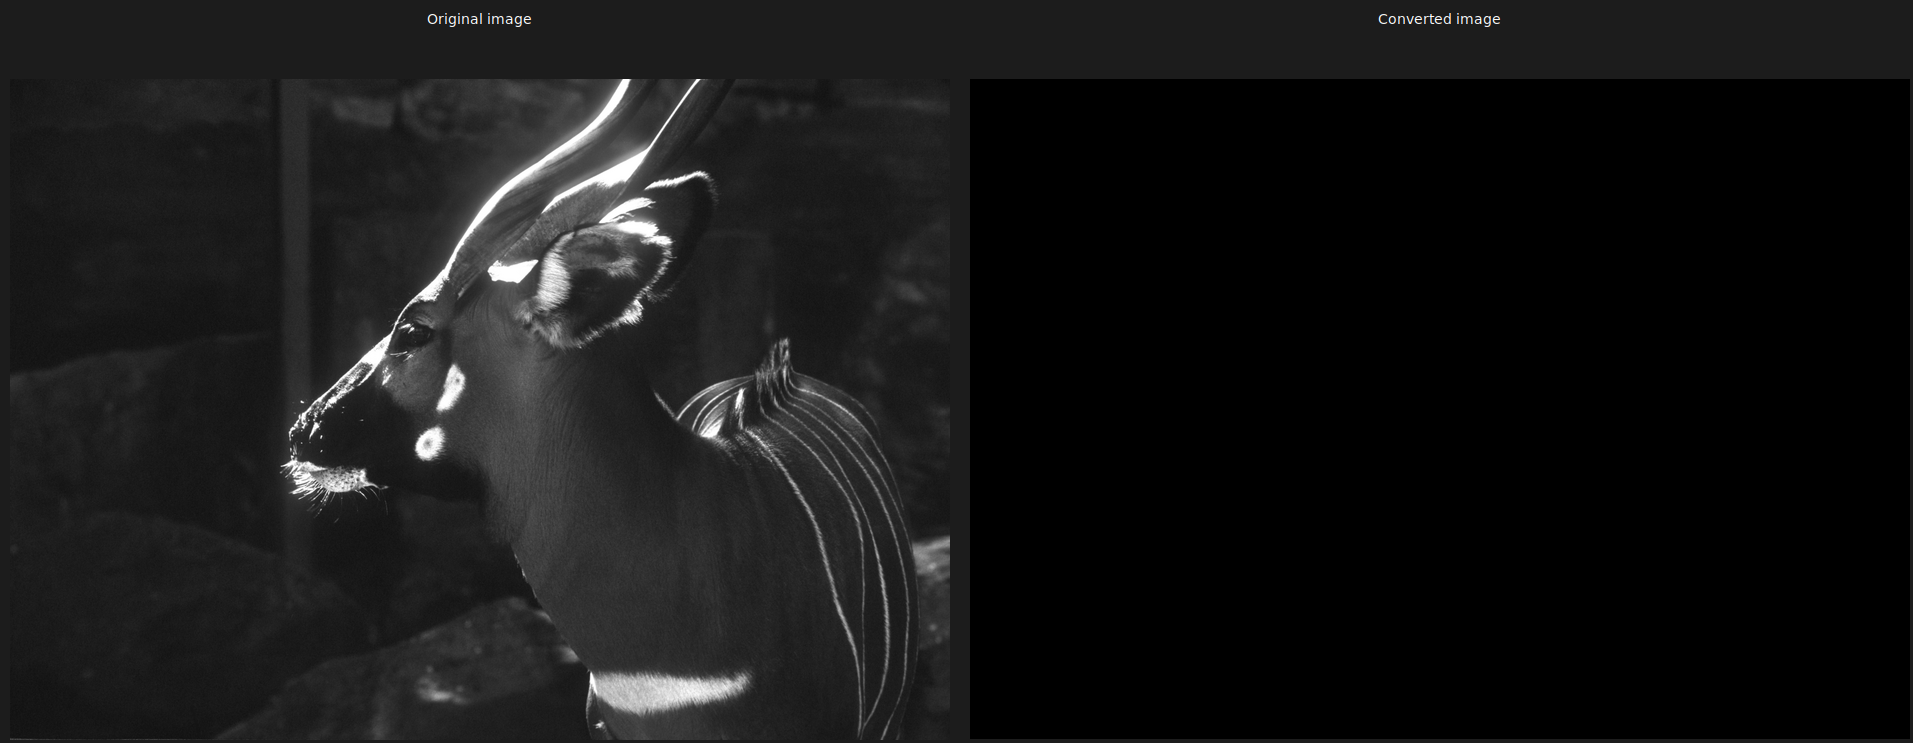
\includegraphics[width=\textwidth]{images/deer-8-0.png}
    \caption{Confronto se $F=8$ e $d=0$.}
    \label{fig:d80}
    \end{center}
\end{figure}

Con $d=1$ si ha che i macroblocchi hanno come colore uniforme la media dei pixel in quel blocco (cfr. figura \ref{fig:d81})

\begin{figure}[!ht]
    \begin{center}
    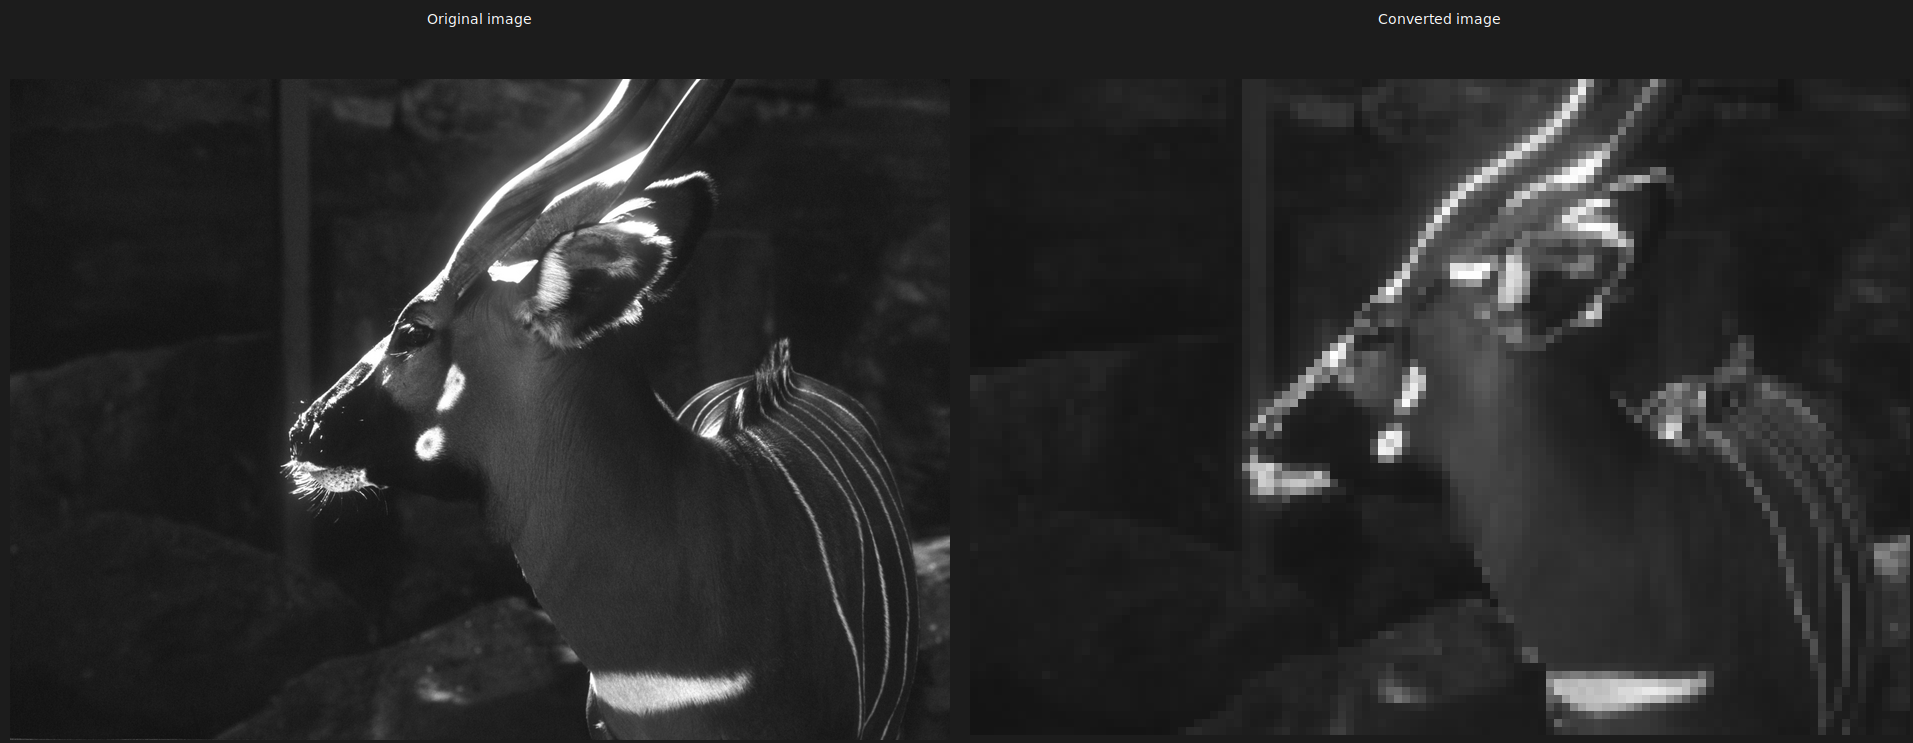
\includegraphics[width=\textwidth]{images/deer-8-1.png}
    \caption{Confronto se $F=8$ e $d=1$.}
    \label{fig:d81}
    \end{center}
\end{figure}

Ponendo $d=3$, otteniamo invece l'immagine in figura \ref{fig:d83}. L'immagine a primo impatto sembra uguale, ma le frequenze tagliate sono molte e zoomando si possono osservare i piccoli quadratini.

\begin{figure}[!ht]
    \begin{center}
    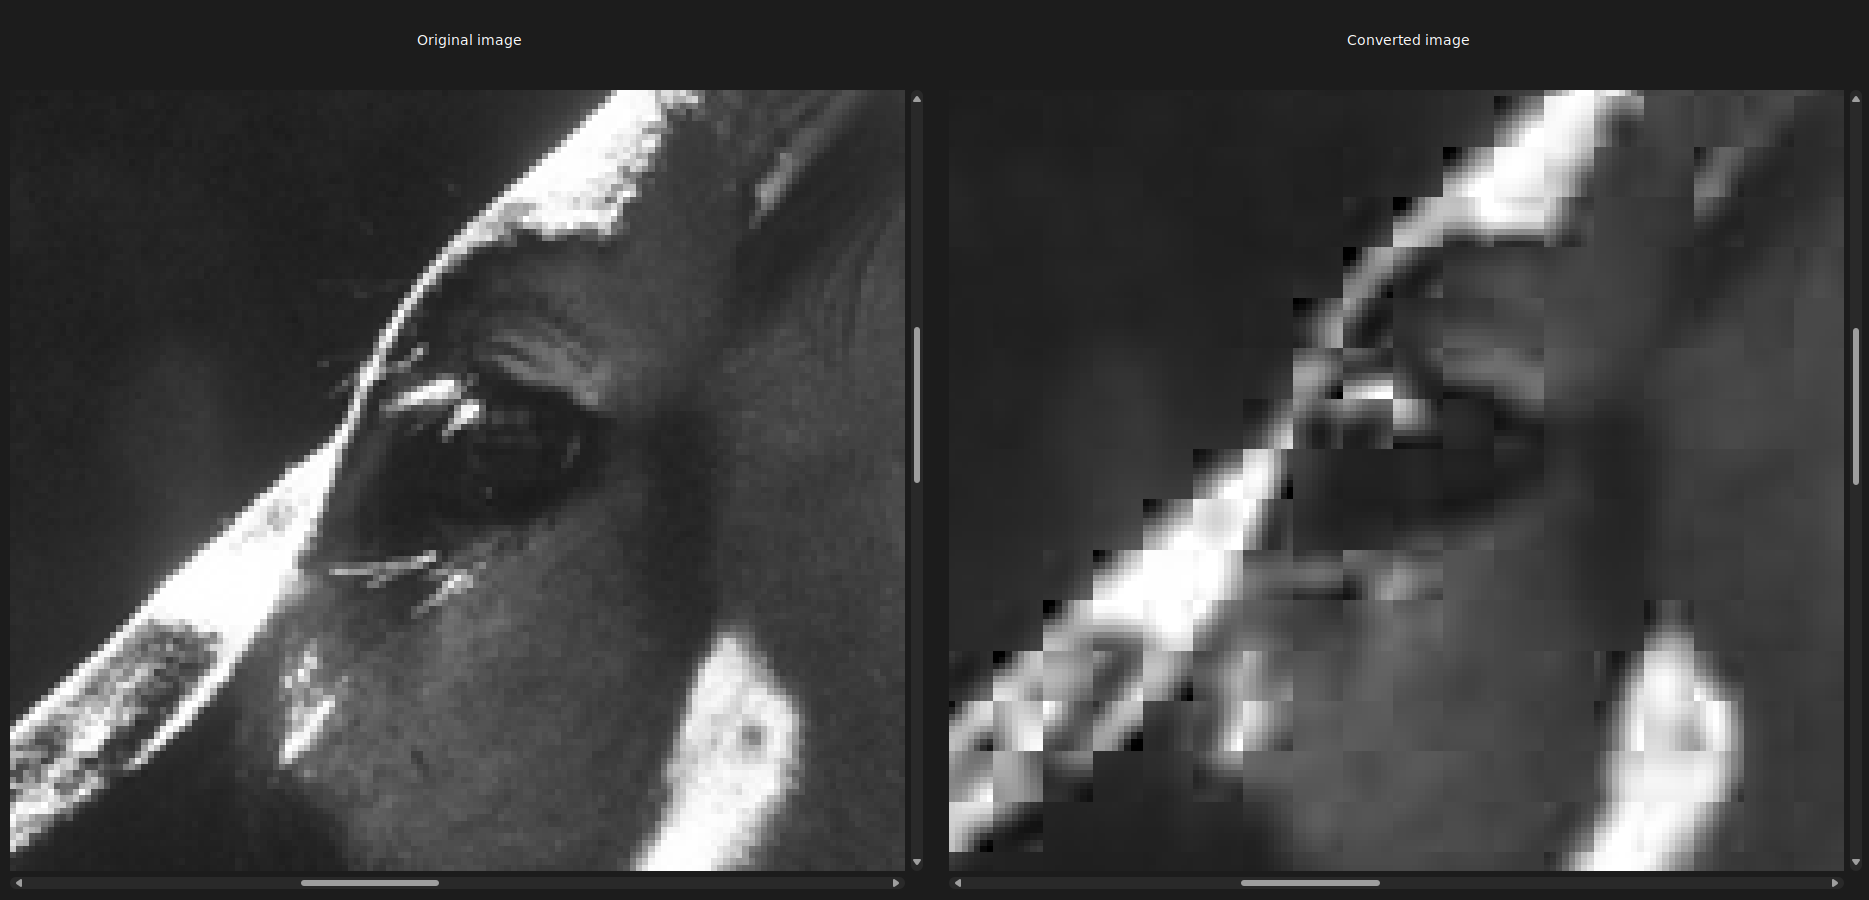
\includegraphics[scale=0.2]{images/deer-8-3-zoom.png}
    \caption{Confronto se $F=8$ e $d=3$ con zoom sul dettaglio.}
    \label{fig:d83}
    \end{center}
\end{figure}

Mantenendo invece tutte le frequenze otteniamo invece l'immagine in figura \ref{fig:d814}, che risulta uguale all'originale.

\begin{figure}[!ht]
    \begin{center}
    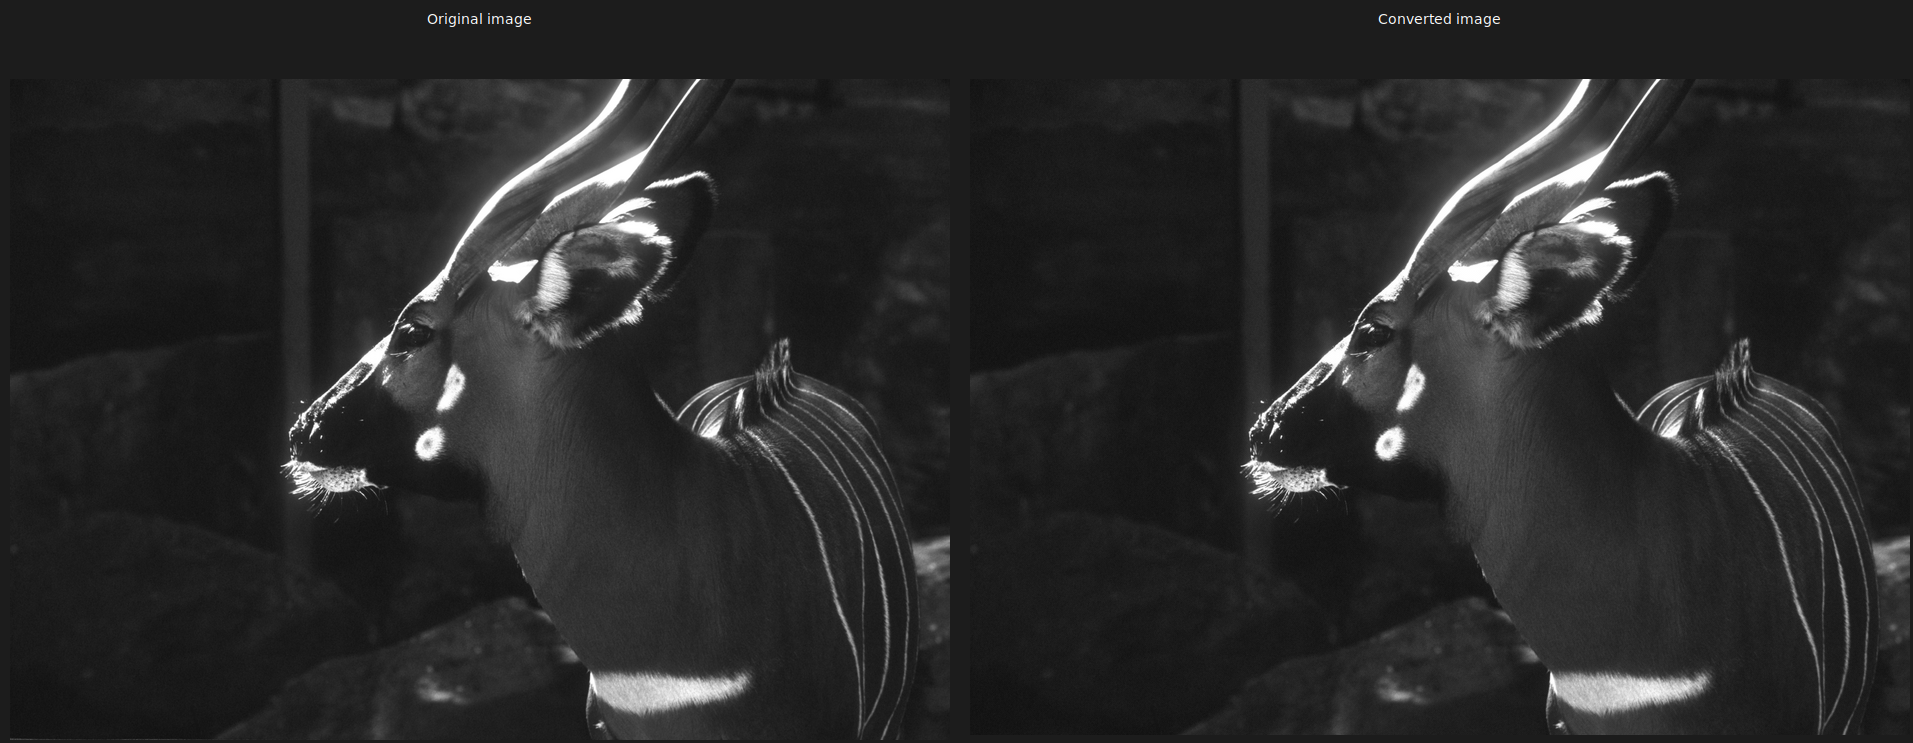
\includegraphics[width=\textwidth]{images/deer-8-14.png}
    \caption{Confronto se $F=8$ e $d=14$.}
    \label{fig:d814}
    \end{center}
\end{figure}

Si prova quindi a impostare una consistente grandezza dei blocchi, dieci volte maggiore di quella precedente, e una soglia di taglio molto bassa. Il risultato è quello in figura \ref{fig:d805}: i blocchi sono evidenti e l'immagine è molto sfocata.

\begin{figure}[!ht]
    \begin{center}
    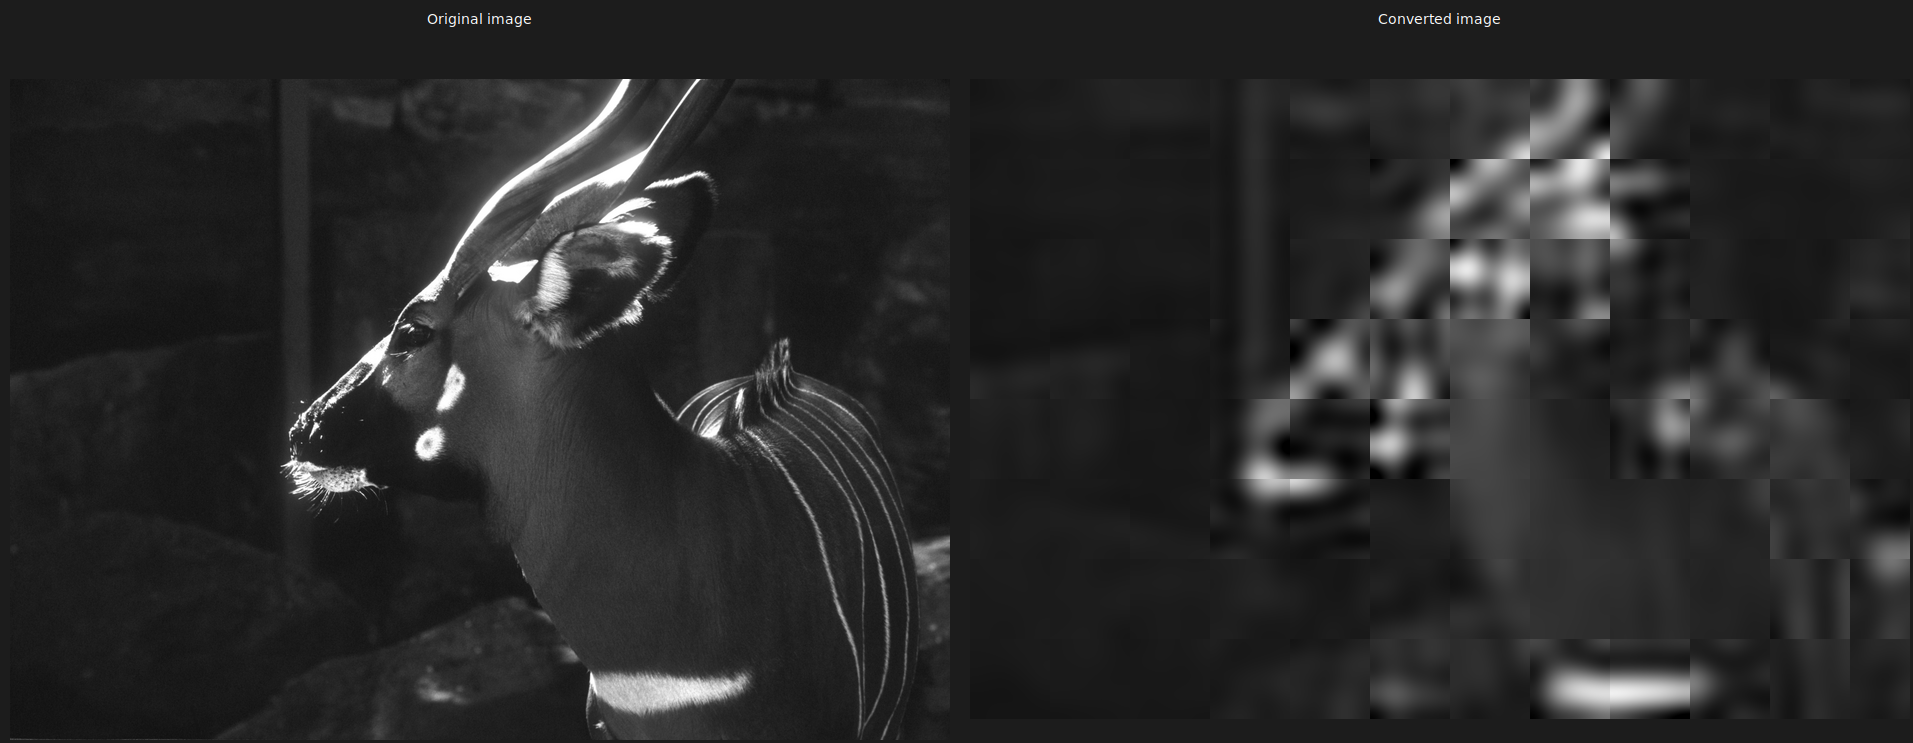
\includegraphics[width=\textwidth]{images/deer-80-5.png}
    \caption{Confronto se $F=80$ e $d=5$.}
    \label{fig:d805}
    \end{center}
\end{figure}

Infine si pone come macroblocco la dimensione del lato minore dell'immagine e $d=1$. Il risultato ottenuto è un unico blocco che ha come colore uniforme la media di tutti i pixel nell'immagine, come si vede in figura \ref{fig:dall1}.

\begin{figure}[!ht]
    \begin{center}
    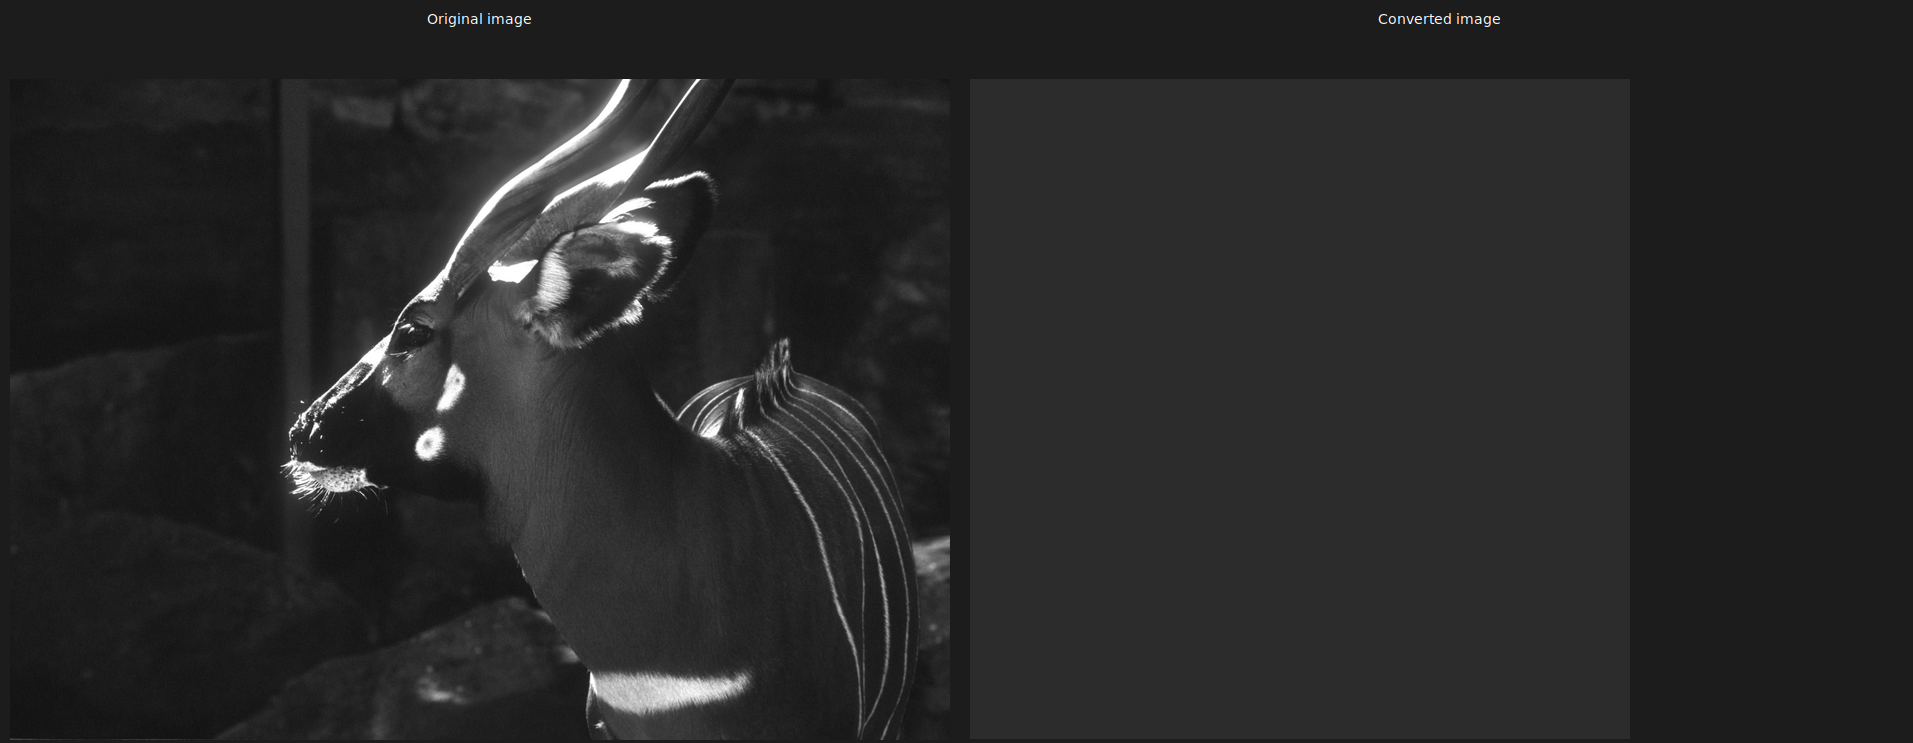
\includegraphics[width=\textwidth]{images/deer-all-1.png}
    \caption{Confronto se il macroblocco è grande quanto il lato minore dell'immagine e $d=1$.}
    \label{fig:dall1}
    \end{center}
\end{figure}

\end{document}
